\documentclass{beamer}
\usepackage{latexsym} 
\usepackage{graphicx}
\usetheme{Warsaw}

\title{Chapter 6}
\subtitle{Model Evaluation and Hyperparameter Tuning}

\begin{document}
\maketitle

\begin{frame}
  \frametitle{How do we know the model is working?}
  \begin{itemize}
  \item Model evaluation
  \item How do we obtain an unbiased estimate of model's performance?
  \item Key concept: estimate model performance on \textbf{unseen} data
  \item Hyperparameters vs. model parameters (e.g. weights)
  \item Model fine-tuning
  \item Performance metrics
  \end{itemize}
\end{frame}

\begin{frame}
  \frametitle{The holdout method}
  \begin{itemize}
  \item Split data into training and test datasets
  \item However, typically we cannot test immediately after training
  \item Need to tune the model to further improve the performance
  \item Select optimial values of hyperparameters
  \item This step is known as \textit{model selection}
  \item A better approach: training set + validation set + test set
  \item Validation set is used for model selection
  \end{itemize}
\end{frame}

\begin{frame}
  \frametitle{The holdout method}
  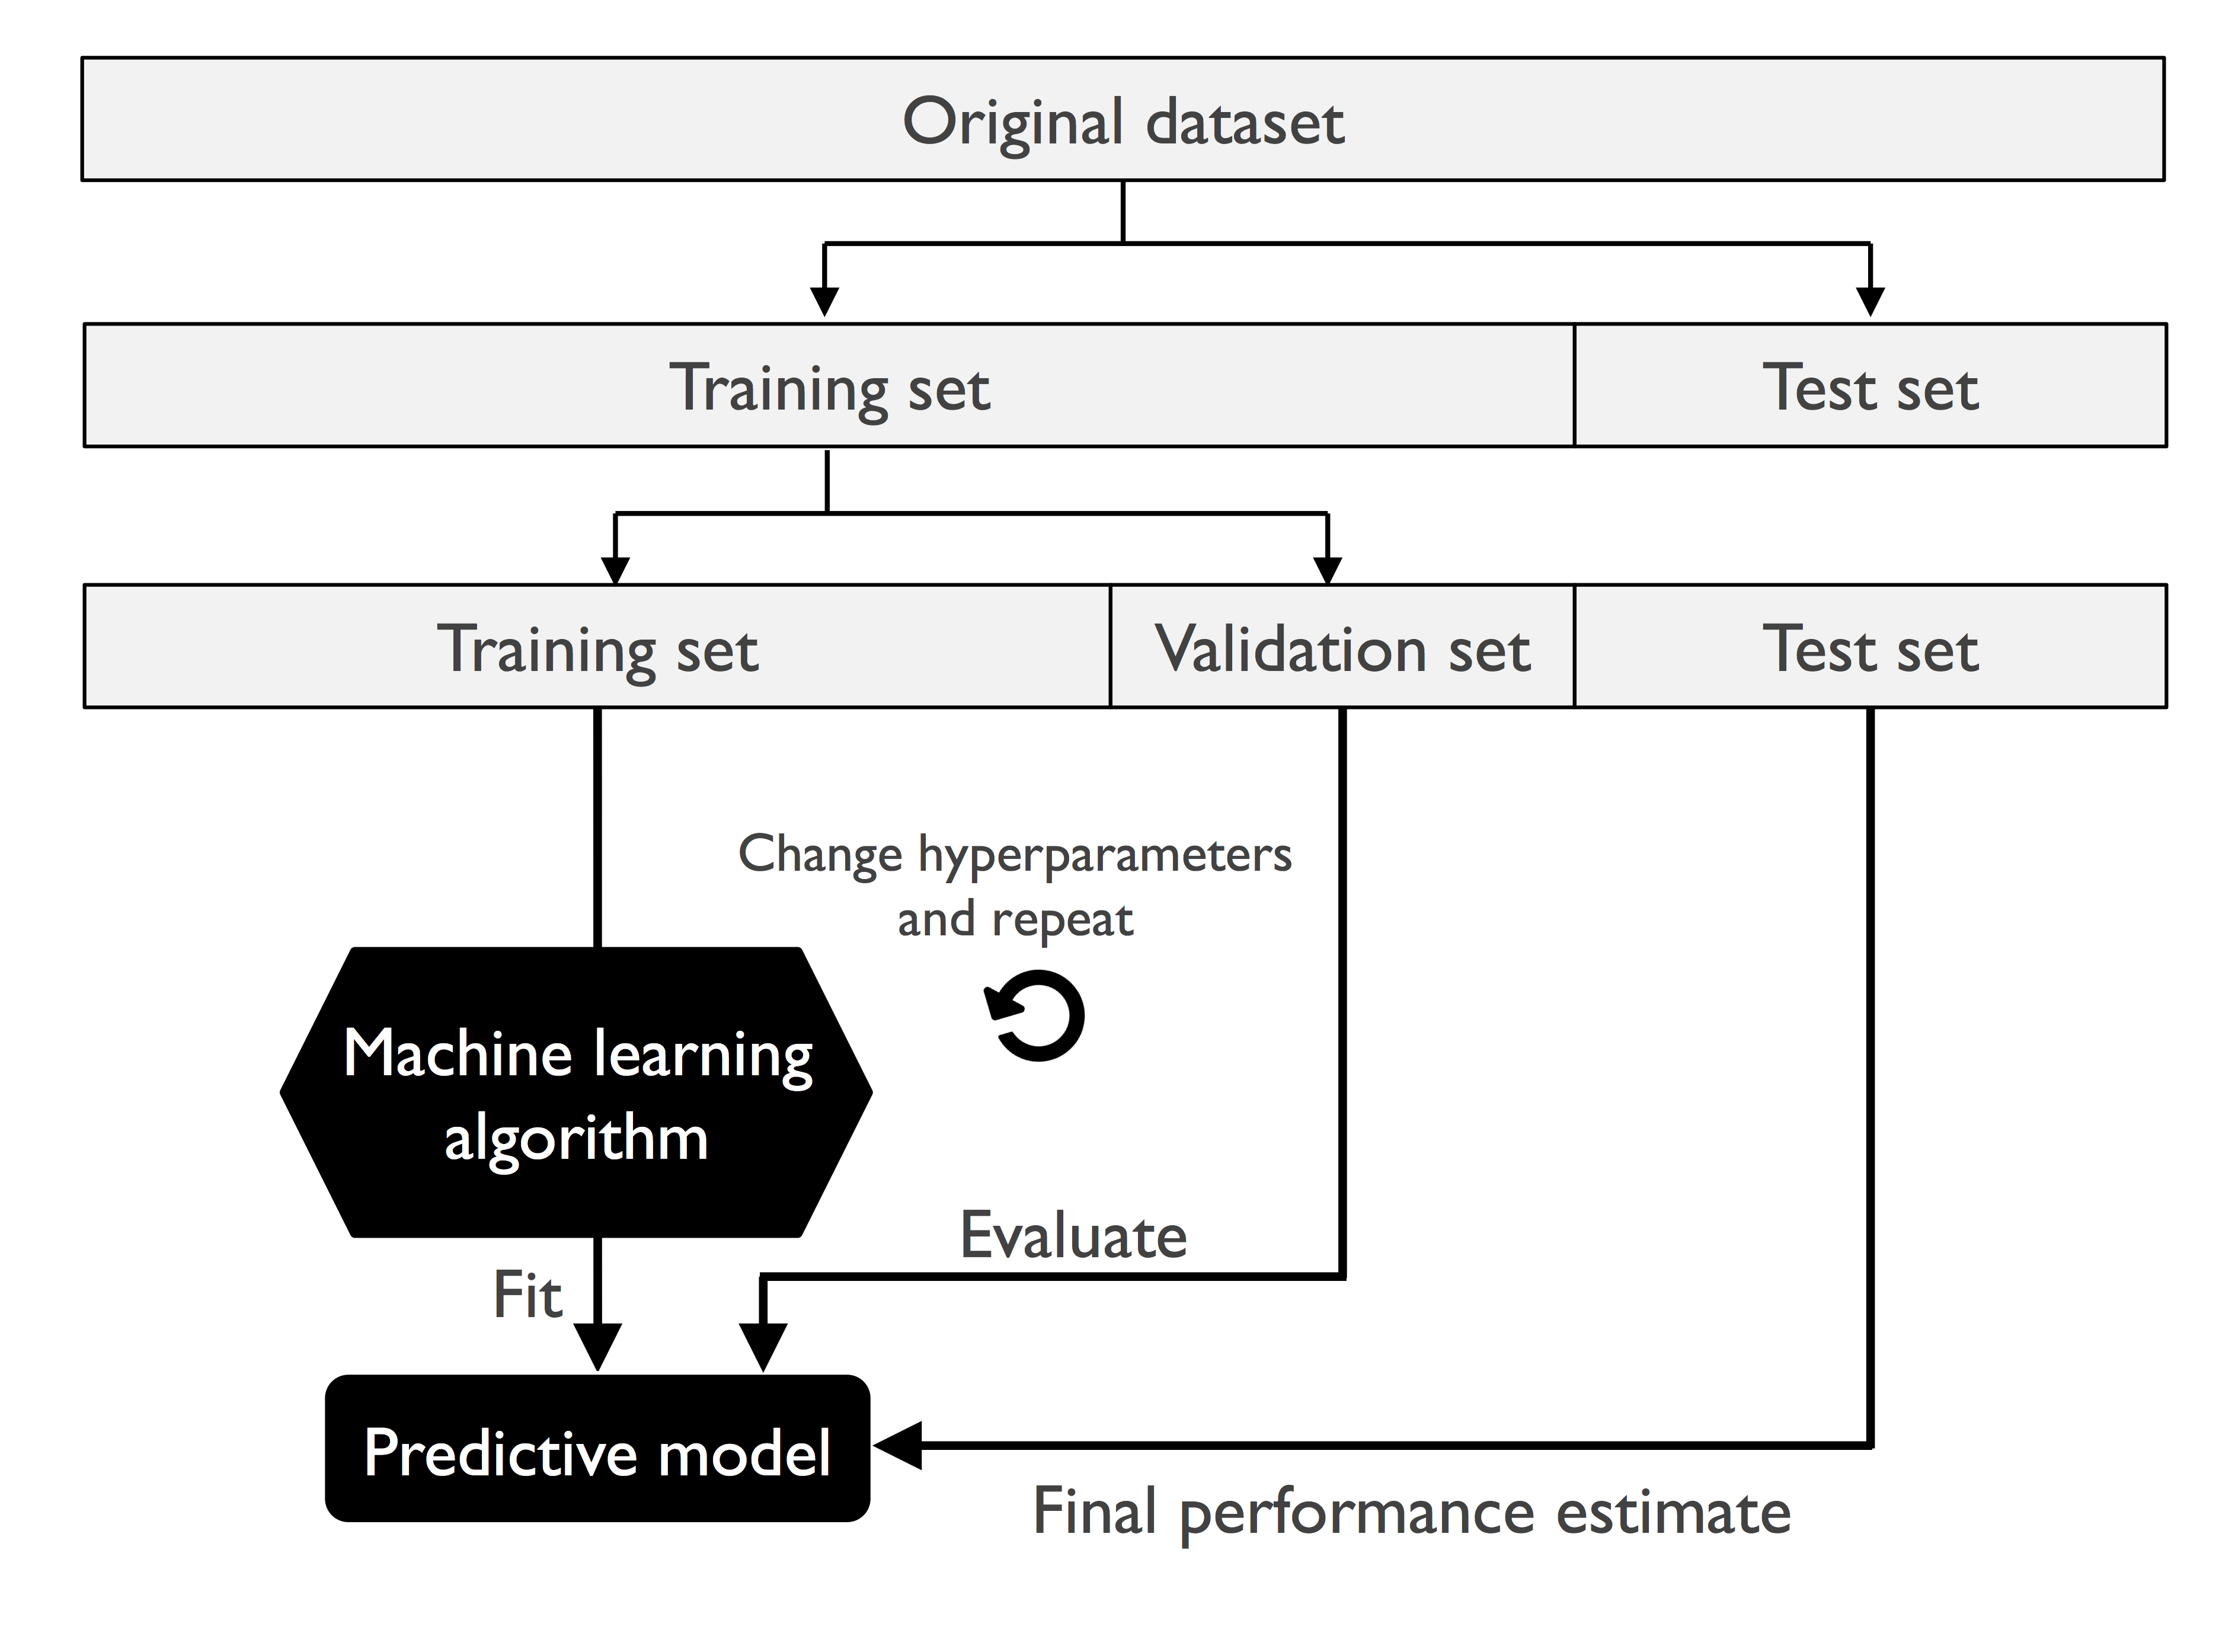
\includegraphics[width=\textwidth]{Code/ch06/images/06_02.png}
\end{frame}

\begin{frame}
  \frametitle{K-fold cross-validation}
  \begin{itemize}
  \item Disadvantage of the holdout method: sensitive to partitioning
  \item Randomly split the training dataset into $k$ folds
  \item Of these, $k-1$ folds are used for training and one for testing
  \item Repeat this procedure $k$ times and average across $k$ folds
  \item Each sample will be part of train and test sets
  \item Lower-variance estimate of the model performance (than holdout)
  \end{itemize}
\end{frame}

\begin{frame}
  \frametitle{K-fold cross-validation}
  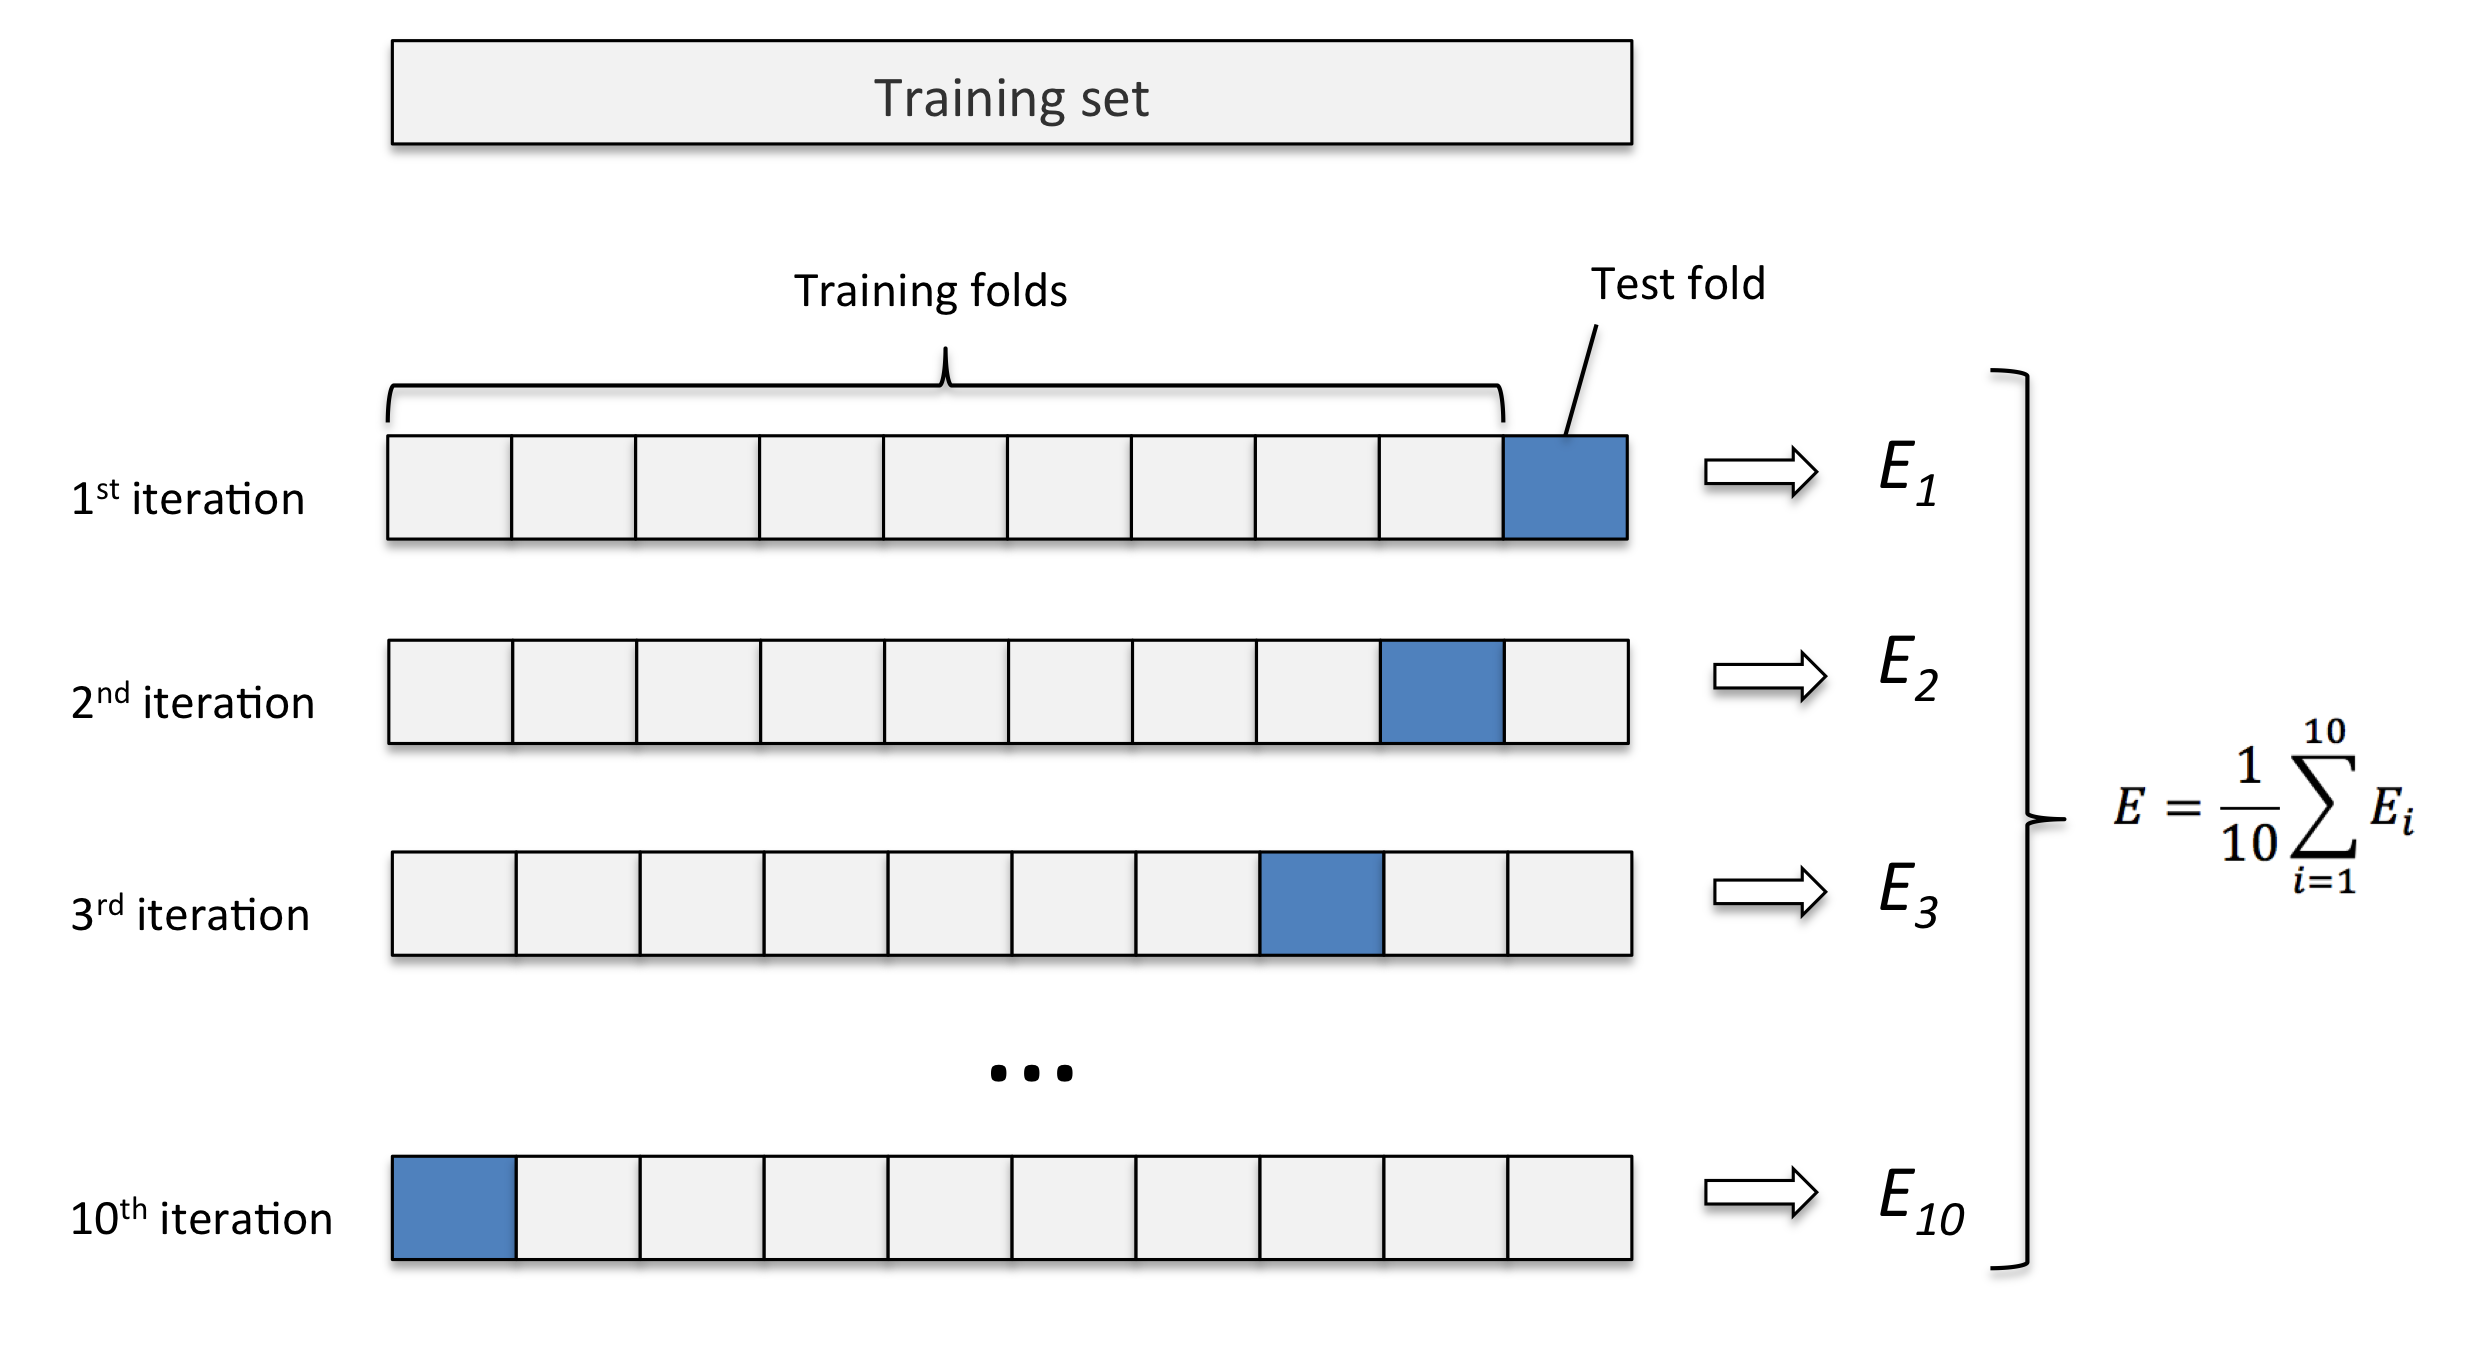
\includegraphics[width=\textwidth]{Code/ch06/images/06_03.png}
\end{frame}

\begin{frame}
  \frametitle{How do we pick the number of folds?}
  \begin{itemize}
  \item The standard value is $k=10$
  \item For small datasets, increase the number of folds
  \item Which will increase the amount of training data
  \item For larger datasets, we can decrease the number of folds
  \item E.g. $k=5$ is a reasonable choice
  \end{itemize}
\end{frame}

\begin{frame}
  \frametitle{Variations on the theme of k-fold cross-validation}
  \begin{itemize}
  \item \textbf{Leave-one-out cross-validation}
    \begin{itemize}
    \item Set the number of folds equal to the number of training samples
    \item Only a single training sample used for testing during each iteration
    \item Recommended approach for very small datasets
    \end{itemize}
  \item \textbf{Stratified k-fold cross-validation}
    \begin{itemize}
    \item Class proportions preserved in each fold
    \item I.e. each fold is representative of the training set
    \item Better performance estimates for imbalanced data
    \end{itemize}
  \end{itemize}
\end{frame}

\begin{frame}
  \frametitle{Grid search}
  \begin{itemize}
  \item Many ML algorithms offer a number of hyperparameters
  \item \href{https://www.csie.ntu.edu.tw/~cjlin/libsvm/}{Link to libsvm command-line arguments}
  \item Find the optimal combination of hyperparameter values
  \item Brute-force exhaustive search of hyperparameter space
  \item Obviously, this can be computationally very expensive
  \end{itemize}
\end{frame}

\begin{frame}
  \frametitle{Performance evaluation metrics}
  \begin{itemize}
  \item We've been using accuracy
  \item Accuracy can be misleading for imbalanced datasets
  \item Need ways to compute the performance for a specific class
  \item Confusion matrix helps visualize different types of errors a classifier can make by reporting the counts of these errors
  \item I.e. true positive (TP), true negative (TN), false positive (FP), false negagive (FN) predictions
  \end{itemize}
\end{frame}

\begin{frame}
  \frametitle{Confusion matrix}
  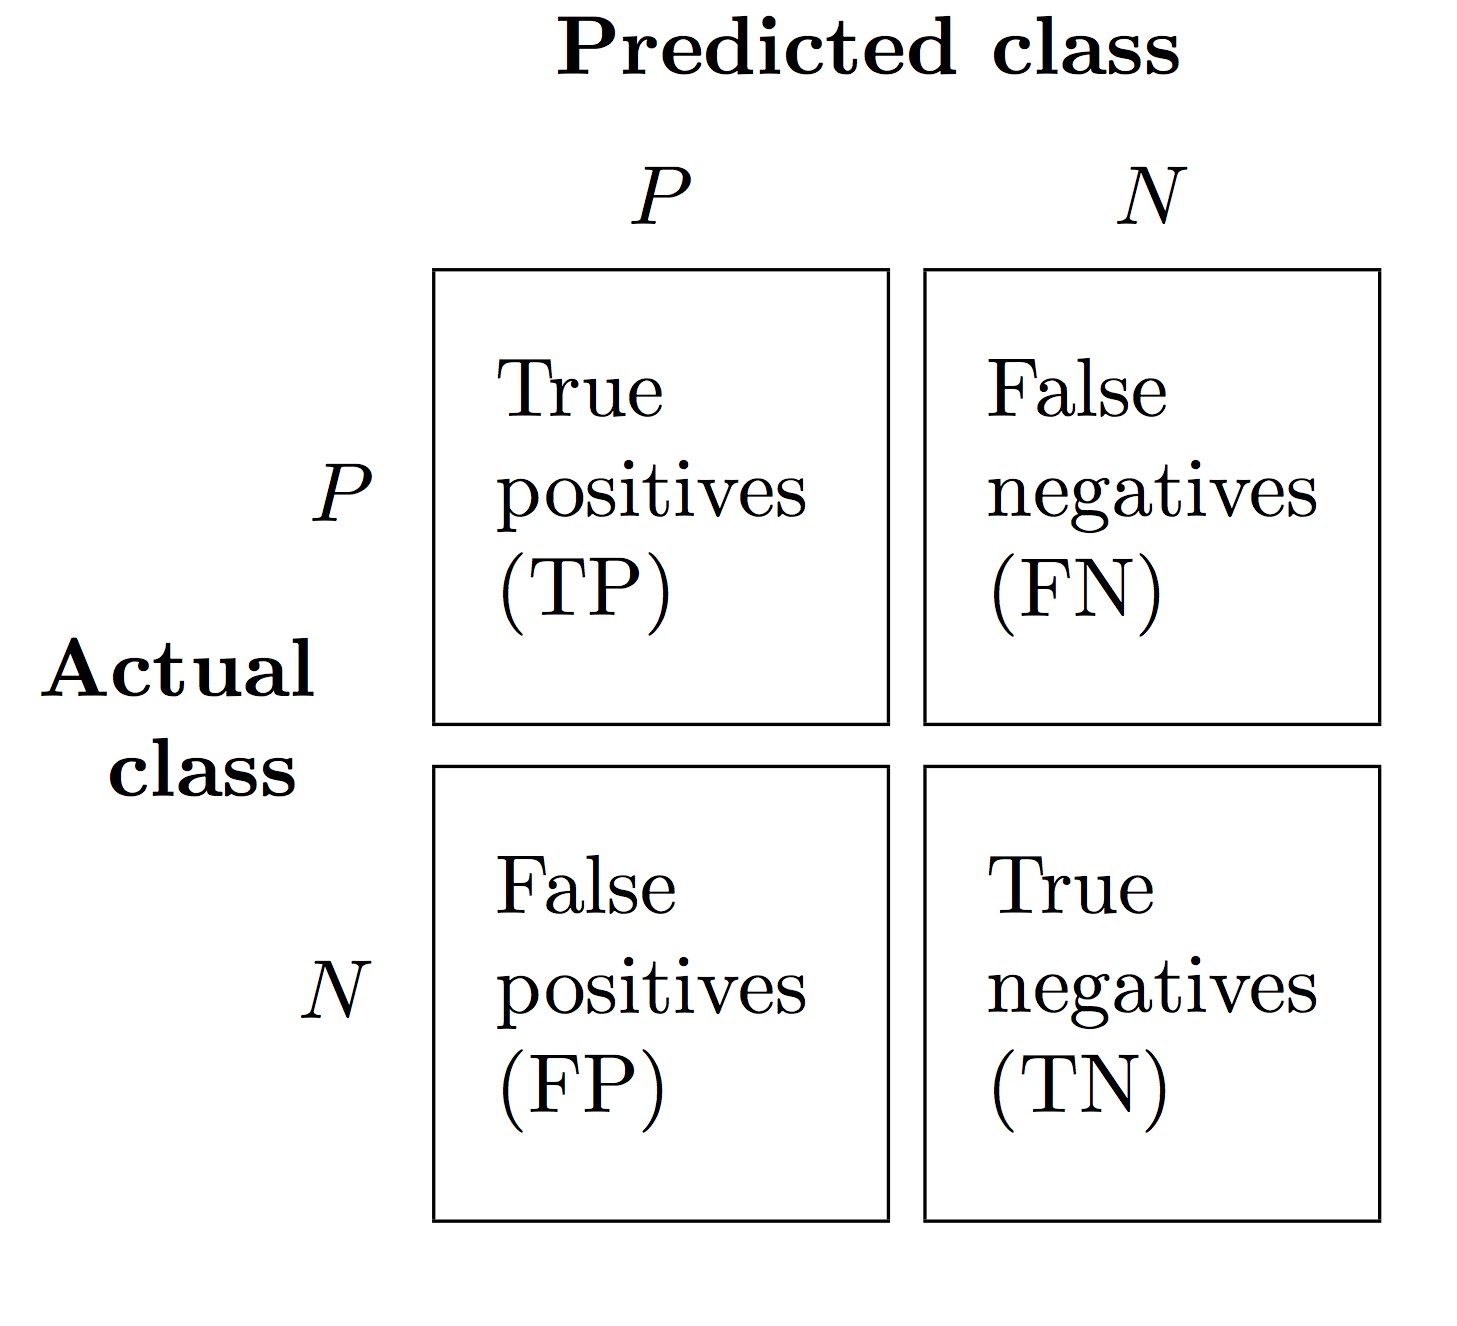
\includegraphics[scale=0.5]{Code/ch06/images/06_08.png}
\end{frame}

\begin{frame}
  \frametitle{Deducing performance metrics from a confusion matrix}
  The error can be understood as the sum of all false predictions divided by the number of total predictions, and the accuracy is calculated as the sum of correct predictions divided by the total number of predictions, respectively:
  \[
  Error = \frac{FP + FN}{FP + FN + TP + TN}
  \]
  The prediction accuracy can then be calculated directly from the error:
  \[
  Accuracy = \frac{TP + TN}{FP + FN + TP + TN} = 1 - Error
  \]
\end{frame}

\begin{frame}
  \frametitle{Precision, Recall, F1}
  \textbf{Precision:}
  \[
  P = \frac{TP}{TP + FP}
  \]
  \textbf{Recall:}
  \[
  R = TPR = \frac{TP}{P} = \frac{TP}{FN + TP}
  \]
  \textbf{F1 score:}
  \[
  \text{F1} = 2 \times \frac{P \times R}{P + R}
  \]
\end{frame}

\begin{frame}
  \frametitle{}
  \begin{itemize}
  \item 
  \end{itemize}
\end{frame}

\end{document}
